\documentclass[a4paper,10pt,twocolumn]{extarticle}
\usepackage[T1]{fontenc}
%\usepackage[utf8]{inputenc}
\usepackage{lmodern}
\usepackage[francais]{babel}
\usepackage{textcomp}
\usepackage[top=2cm,bottom=2cm,left=2cm,right=2cm]{geometry}
\usepackage{amsmath}
\usepackage{amssymb}
\usepackage{mathrsfs}
\usepackage{float}
\usepackage{icomma}
\usepackage{gensymb}
\usepackage{graphicx}
\usepackage{subcaption}
\usepackage[font=sf, labelfont={sf,bf}, margin=1cm]{caption}
\usepackage[french,onelanguage,ruled,lined]{algorithm2e} % pour pseudo code
\usepackage{array}
\usepackage{titlesec, fontspec, titling}

% Specify different font for section headings
\newfontfamily\headingfont[]{GillSans}
\titleformat*{\section}{\LARGE\headingfont}
\titleformat*{\subsection}{\Large\headingfont}
\titleformat*{\subsubsection}{\large\headingfont}
\renewcommand{\maketitlehooka}{\headingfont}

\pretitle{\begin{flushleft}\fontsize{22}{18}}
\posttitle{\par\end{flushleft}\vskip 0.5em}
\preauthor{\begin{flushleft}\Large \lineskip 0.5em}
\postauthor{\par\end{flushleft}}
%\predate{\begin{flushleft}\large}
%\postdate{\par\end{flushleft}}
\setlength{\droptitle}{-1cm}
\title{\textsf{Implémantation d’un système de détection et de reconnaissance faciale}}
\author{Alexandre Bonhomme\\ {\normalsize Université Paul Sabatier, Toulouse}\\
Florent Maufras\\ {\normalsize EFREI, Paris}\\
Timothée Planté\\ {\normalsize EISTI, Pau}\\}% \small{BONA20128906}}
\date{}

\begin{document}
\maketitle
\section{Introduction}
La reconnaissance faciale est actuellement un domaine en plein essort. Elle rentre petit à petit dans nos vies au travers de nos téléphones mobiles ou de nos ordinateurs portables par exemple. Malgré l'amélioration du taux de détection elle reste actuellement l'objet de nombreuses études.

L'objectif de notre projet sera de mettre en oeuvre un système complet permettant la détection et la reconnaissance de visage issue de plusieurs bases de données. Pour ce faire nous implémenterons différents algorithmes de reconnaissance et nous utiliserons la bibliothèque OpenCV \cite{opencv} et son implémentation de l'algorithme de Viola \& Jones pour la détection de visage.

\section{Algorithmes mis en oeuvre}
Au cours de notre projet nous avons confronté différents algorithmes afin de tester leurs aptitudes sur plusieurs ensembles de données différents.

\subsection{K Plus Proches Voisins et Fenêtres de Parzen}
L'algorithme des <<K plus proches voisins>> (KPPV) utilise le voisinage du point de test afin de déterminer sa classe. C'est la classe majoritaire parmi ces $K$ points qui sera attribuée au point de test (\ref{fig:knn}).

Pour cet algorithme il n'y a pas d'apprentissage des paramètres sur l'ensemble d'entrainement, seulement une optimisation des l'hyperparamètres $K$ sur l'ensemble de validation.
\begin{figure}[H]
  \begin{center}
    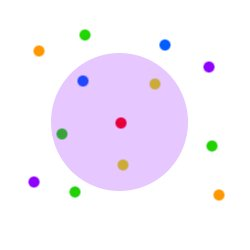
\includegraphics[width=100pt]{images_rapport/KNN.png}
    \caption{K Plus Proches Voisins}
    \label{fig:knn}
  \end{center}
\end{figure}
Dans la Figure~\ref{fig:knn} le point de test (en rouge) va recevoir comme prédiction la classe jaune car c'est elle la plus présente dans les $K = 4$ voisins les plus proches. Le disque ici n'est que représentatif pour mettre en évidence les voisins. Les points voisins peuvent être à une distance plus ou moins importantes de notre point test.

\subsubsection{Extension avec les fenêtres de Parzen}
L'application que l'on a fait ici de Parzen nous permet de pondérer les points du voisinage. Plus un point sera distant du point à l'étude plus son poids sera faible. Cela est calculé à partir d'une gaussienne centrée sur le point à l'étude et d'une largeur fixée par $\sigma$, dans notre cas $\sigma$ sera fixé par l'utilisateur.

\subsection{Réseau de Neurones}
Le réseau de neurone utilisé dans ce projet est de type Perceptron Multicouche. Ce modèle est entrainé par descente de gradient de bacth sur un ensemble d'entrainement afin d'optimiser les paramètres du réseau en réduisant le risque empirique régularisé. On tâchera ensuite d'optimiser les hyperparamètres de contrôle de capacité sur un ensemble de validation séparé.
\begin{figure}[H]
  \begin{center}
    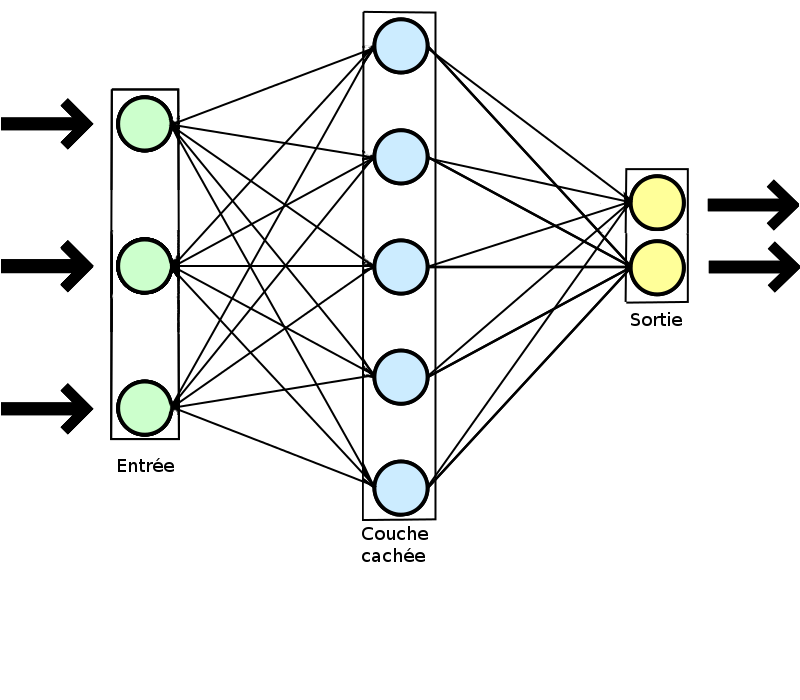
\includegraphics[width=220pt]{images_rapport/Neural_network.png}
    \caption{Réseau de neurones}
    \label{fig:nnet}
  \end{center}
\end{figure}
Dans notre cas nous utiliserons une architechture monocouche (cf. Figure~\ref{fig:nnet}) et une pénalité de type <<weight decay>> (\ref{eq:penalité}) pour la régularisation car elle défavorisera les poids les plus lourds lors de l'apprentissage des paramètres. 
\begin{align}\label{eq:penalité}
  \Omega(\theta) = \| \mathbf{W}^{(1)} \|^2 + \| \mathbf{W}^{(2)} \|^2
\end{align}
Cette pénalité sera pondérée par un hyperparamètre $\lambda$.

\subsection{Algorithme de Viola et Jones}
Afin d'effectuer efficacement la détection de visage nous avons utilisé une implémentation de l'algorithme de Viola et Jones \cite{viola01} proposé par la célèbre bibliothèque de traitement d'image \textit{OpenCV} \cite{opencv}.

Cet algorithme est basé sur le principe de <<boosting>> qui consiste à assembler plusieurs classifieurs faibles afin d'obtenir un classifieur à forte capacité. Plutôt que de travailler directement sur les pixels de l'image, Viola P. et Jones M., introduisent des caractéristiques appelées <<pseudo-Haar>> fortement inspirées des ondelettes de Haar. De plus il utilise une variante d'un algorithme de boosting très célèbre qui est l'<<AdaBoost>>.
\begin{figure}[H]
        \centering
        \begin{subfigure}[b]{110pt}
                \centering
                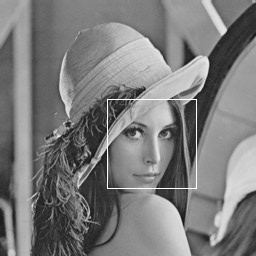
\includegraphics[width=110pt]{images_rapport/lena.png}
                \caption{Image initiale}
                \label{fig:lena}
        \end{subfigure}
        \begin{subfigure}[b]{110pt}
                \centering
                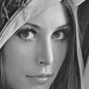
\includegraphics[width=60pt]{images_rapport/lena_face.png}
                \caption{Visage extrait}
                \label{fig:lena_face}
        \end{subfigure}
        \caption{Détection d'un visage par l'algorithme de Viola et Jones \cite{viola01} \label{fig:viola_detect}}
\end{figure}
Cette technique est particulièrement efficace et offre d'excelents résultats pour la détection de visages (cf. Figure~\ref{fig:viola_detect}) et par extension la détection de motifs (ou d'objets) au sein d'une image.

\section{Ensembles de données utilisés}
Afin d'entrainer nos algorithmes et de mesurer leurs perfomances nous avons essentiellement utilisé deux jeux de données.

\subsection{Our Database of Faces (ORL \cite{orl})}
Le premier ensemble de données utilisé est issu des laboratoires de l'entreprise \textit{AT\&T}. C'est un ensemble de taille moyenne qui regroupe au total 40 sujets différents avec 10 images par sujet. Les photos ont été prises sous différentes postures et durant plusieurs années et ont une taille de $92 \times 112$ pixels.

Les images sont en niveaux de gris (NdG) et au format PGM.

\subsection{Labeled Faces in the Wild Home (LFW \cite{lfw})}
Pour le second jeu de données, il est mis a diposition par l'université du Massachusetts et il s'agit de photographies tirées d'Internet et sur lesquels l'algorithme de Viola et Jones \cite{viola01} a été appliqué afin d'obtenir une image de taille $250 \times 250$ pixels centré sur le visage.

Cet ensemble est relativement grand il contient 13233 images de 5749 sujets différents. Les images sont en couleur et au format JPG.

\subsection{Prétraitements des données}
\subsubsection{Cas particulier : l'ensemble LFW}
Contrairement à l'ensemble ORL, LFW nécessite des prétraitement supplémentaires. En effet, nous avons utilisé l'ensemble LFW pour simuler une entrée réelle dans notre système. Pour ce faire nous avons appliqué l'algorithme de Viola et Jones afin de détecter les visages au sein des images présentes dans l'ensemble.\\
Nous avons ainsi pu extraire (après divers traitements de redimensionnement) une image de taille $92 \times 115$ pixels en plusieurs NdG.

\subsubsection{Cas général}
Appartir des images en différents NdG nous construisons une représentation vectorielle de celle-ci (cf. Figure~\ref{fig:vectorisation}).
\begin{figure}[H]
  \begin{center}
    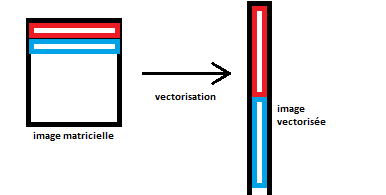
\includegraphics[width=220pt]{images_rapport/vectorisation.png}
    \caption{Vectorisation d'une image}
    \label{fig:vectorisation}
  \end{center}
\end{figure}
Cependant cette représentation est très lourde car elle contient de nombreuses caractéristiques. Afin de reduire la dimentionalité de nos données d'entrainement nous avons appliqué l'agorithme du \textit{PCA} (<<Principal Components Analysis>>), plus connu sous le nom de <<Eigenfaces>> \cite{turk91} lorsqu'il est appliqué à la reconnaissance facial.

\subsubsection{Réduction de la dimentionnalité : PCA}
Nous avons implémenté le PCA dans ca forme classique.\\
On normalise l'ensemble de données en sustrayant le <<visage>> moyen :
\begin{align}
  X_N = X - \bar{x}
\end{align}
A la suite de quoi nous utilisons une <<astuce mathématique>> qui consiste à calculer la Décomposition en Valeurs Singulières (ou SVD pour <<Singular Value Decomposition>>) afin de déterminer les vecteurs propres de la matrice de covariance. On obtient alors :
\begin{align}
  X_N = USU^T
\end{align}
Ou les colonnes de $U$ contiennent les vecteurs propres et $S^2$ les valeurs propres associées. On ne conserve alors qu'un nombre $M$ de vecteurs propres (ie. $M$ colonnes de la matrice $U$). Après réduction du nombre de colonnes on obtient une matrice $U^{\prime}$ (aussi appelée, dans notre cas, <<Eigenspace>>) dans laquelle on projete l'ensemble de données $X$ afin de déterminer la matrice de poids $W$ associée :
\begin{align}
  W = \langle (U^{\prime})^T , X \rangle
\end{align}
Ainsi, pour chaque nouvel exemple $x$ on calculera son vecteur de poids $w$ par projection dans le Eigenspace $U^{\prime}$.

\section{Vérifications des algorithmes}
Afin de vérifier le bon fonctionnement des algorithmes implémentés nous avons mis en oeuvre quelques procédures de vérification.

\subsection{Perceptron Multicouche}
Pour le réseau de neurones nous avons vérifié nos résultats sur l'ensemble de données deux dimensions <<MOONS>> et nous avons obtenu les résultats de la Figure~\ref{fig:verif_nnet}.
\begin{figure}[H]
        \centering
        \caption{Vérification du réseau de neurones}\label{fig:verif_nnet}
        \begin{subfigure}[b]{220pt}
                \centering
                \caption{Risque empirique}
                \includegraphics[width=220pt]{images_rapport/nnet_risque.png}
        \end{subfigure}
        \begin{subfigure}[b]{220pt}
                \centering
                \caption{Erreur de classification}
                \includegraphics[width=220pt]{images_rapport/nnet_erreur_classif.png}
        \end{subfigure}
        \begin{subfigure}[b]{220pt}
                \centering
                \caption{Frontières de décision}
                \includegraphics[width=220pt]{images_rapport/nnet_fontieres.png}
        \end{subfigure}
\end{figure}

\subsection{Détection de visages}
Pour vérifier le bon fonctionnement de la détection de visage nous avons effectué des essais préalables des images de test telle que celle de la Figure~\ref{fig:viola_detect}.

\section{Résultats}
\subsection{ORL}


\subsection{LFW}

\section{Particularités du projet}
Une des caractéristiques de notre projet est qu'il a été réalisé par une équipe de trois personnes ayant suivi des formations différentes. De plus nous avons dû mettre en place un gestionnaire de version (Git) afin de pouvoir travailler efficacement malgré nos diponibilités très disparates.

L'usage du langage Python a aussi ajouté son lot de complications car nous avons tous les trois découvert ce langage au début du semestre.

La dernière difficulté, et non des moindres, concerne le sujet en lui-même. En effet, la reconnaissance faciale est un sujet d'étude actuel et aucun système n'est encore réellement fiable dans ce domaine.

Nous avons cependant obtenu des résultats concluants sur le jeu de données ORL, confirmant l'efficacité de notre programme dans le domaine de la reconnaissance faciale .

Ce dernier se montre moins concluant lorsqu'il s'agit d'un jeu de données comportant des portaits moins conventionnels comme le jeu de données LFW contennant nombre d'éléments perturbatoires (lunettes, micros, certaines images présentant aussi plusieurs visages), et marque ainsi une perspective d'améliorations futures.


\section{Conclusion}


\begin{thebibliography}{9}
\bibitem{turk91}
  \bsc{Turk M. and Pentland A.}, 
  \emph{Eigenfaces for recognition}.
  J. Cognitive Neuroscience,
  1991. 
\bibitem{orl}
  \bsc{Samaria F. and
      Harter A.}, 
  \emph{Parameterisation of a stochastic model for human face identification}.
  2nd IEEE Workshop on Applications of Computer Vision,
  1994.
\bibitem{opencv}
  \bsc{Bradski G.}, 
  \emph{The OpenCV Library}.
  Dr. Dobb's Journal of Software Tools,
  2000.
\bibitem{viola01}
  \bsc{Viola P. and 
      Jones M.}, 
  \emph{Rapid object detection using a boosted cascade of simple features}.
  Computer Vision and Pattern Recognition,
  2001.
\bibitem{lfw}
  \bsc{Huang G. B.,
       Ramesh M.,
       Berg T. and 
       Learned-Miller E.}, 
  \emph{Labeled Faces in the Wild: A Database for Studying Face Recognition in Unconstrained Environments}.
  University of Massachusetts, Amherst,
  2007.

\end{thebibliography}
\end{document}
